% -----------------------------------------------
% Vlastní text práce (kapitoly práce)
% -----------------------------------------------

% -----------------------------------------------
\chapter{Monitoring system}
% -----------------------------------------------
As was mentioned before, the quality of the fluorescence detection depends on athmospheric conditions and a durability of detection parts is also dependent on exposure to these effects. Thus it is highly advised to monitor them and plan shifts according to these conditions. To capture athmospheric data, we construted a monitoring system - a meteostation, which we describe in this chapter.
% -----------------------------------------------
\section{Monitoring of multiple FAST telescopes}
% -----------------------------------------------
The main goal was to develop a monitoring system for multiple FAST telescopes, which is capable of acquiring data of temperature, humidity, wind speed and direction, raining and light exposure. These data have to be easily accessible, so it is necessary to store them in some database, which could be accessed throughout the network. 
\par
The data could be used by operator when controlling the telescope or later in a complex analysis of detection events and calibration measurements. For example, the operator must be sure that there is no light source outside before he executes command to open the shutter of the telescope's hut. To obtain this information, he checks for the measured value from an ambient light sensor, which is a part of monitoring system.
\par
% -----------------------------------------------

\section{Control units and sensors}
% -----------------------------------------------
Central control unit is a RPi, which collects data from other STM32 nucleos. For every FAST telescope there is one STM32 nucleo equipped with sensors, which is connected to the RPi via CAN bus. The operation scheme could be seen on (fig. \ref{opScheme}). The RPi itself takes care of ultrasonic wind sensor and a rain sensor, because both wind and rain are same for every telescope. The Nucleos have connected dallas DS18B20 thermometers (1-Wire), BME230 temperature, humidity and pressure sensor(I2C) and an ambient light sensor (OPT3001) through an optoclick module. Additional possibility is also to include induction sensor catch failures in shutter opening/closing.


\begin{figure}[H]
 \centering
 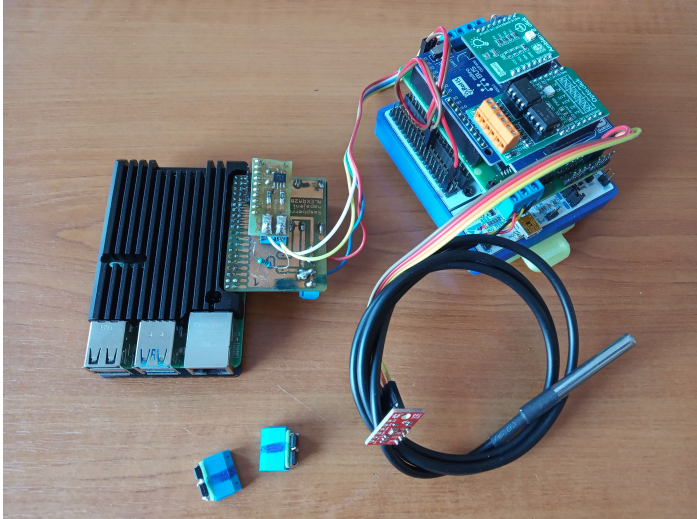
\includegraphics[scale = 0.5]{./pictures/Metostation}
 \caption{RPi and STM32 with sensors.}
 \label{MonNuc}
\end{figure}


\begin{figure}[H]
 \centering
 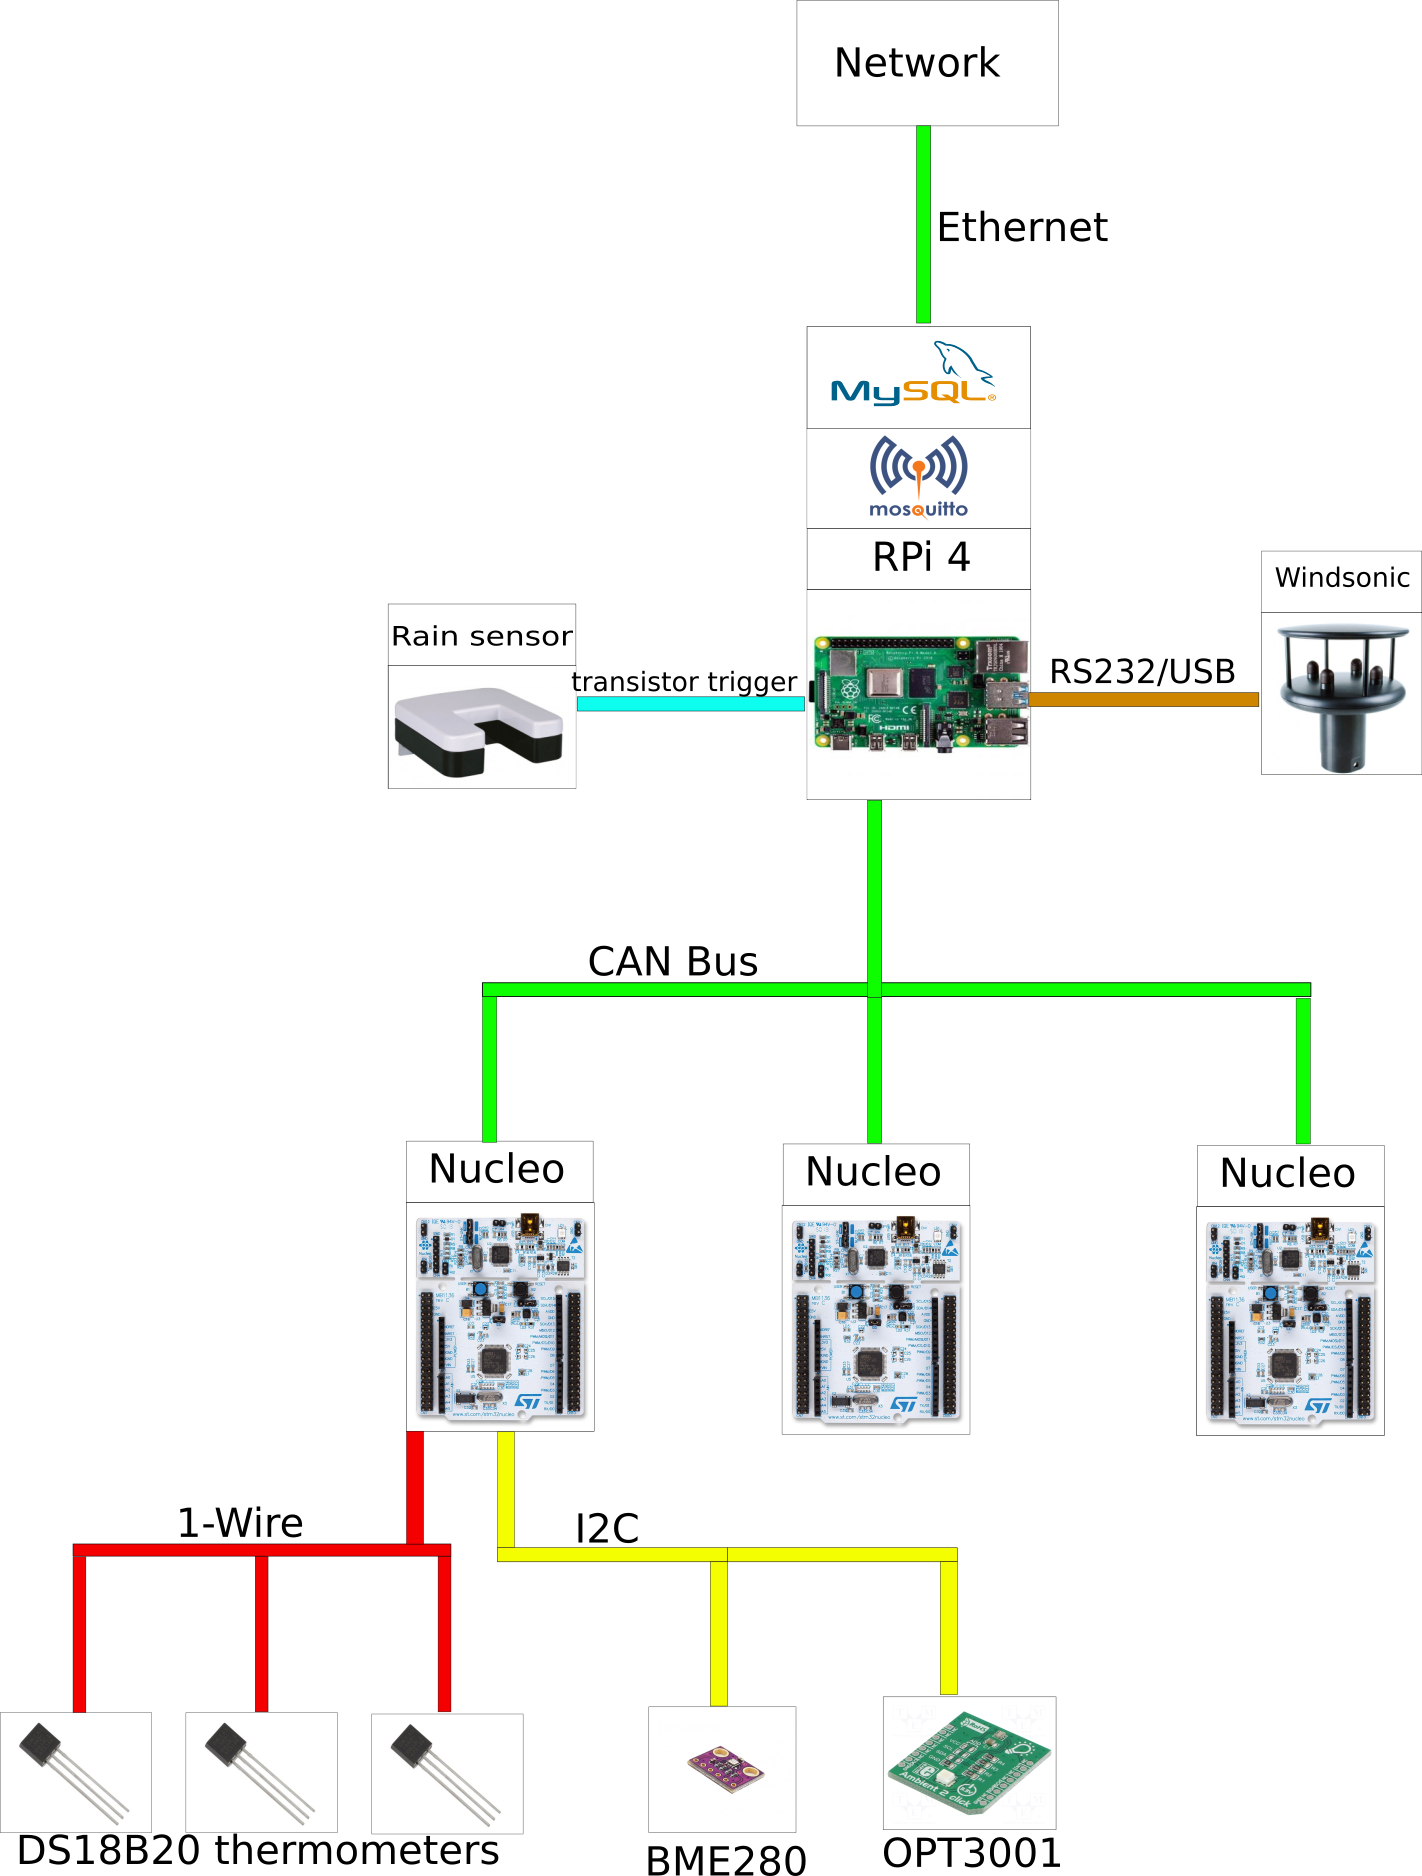
\includegraphics[scale = 0.3]{./pictures/monitoringScheme}
 \caption{Operation scheme of the monitoring system.}
 \label{opScheme}
\end{figure}




%------------------------------------------------

\section{Software system}
% -----------------------------------------------
For this application, where is not essential to achieve fast sampling and do some fast responses, we decided to use python fo RPi and micropython for STM32 nucleo. These languages offer us libraries and easy programming for some of our sensors, however in a cost of speed and memory (compared to C/C++ for example).
\par
The data reading scripts are scheduled by classic linux's tool - crontab.


\par
The main part of software communication between RPi (and RPi's internal processes) and Stm32 nucleos is done throught the MQTT Mosquitto server, which runs on RPi. Nowadays the MQTT is a useful service used in automatization processes, where the many messages from various devices are sent and received simultaneously. The processes coud have three roles - publisher, subscriber and broker (in our case done by MQTT itself). The publisher process sends data packet with theme to broker. The broker calls all subscribers of this theme and passes them the data packet \cite{MqttServ}. The processes must be programmed to communicate with MQTT service, which could be done by using various MQTT libraries. The MQTT scheme could be in our case specified in following way: The running scripts (representing processes for MQTT) for data acquisition (Wind, rain, nucleo data transfer) are programmed as publishers and publish values of specified sensors with theme related to their names and types in specified intervals. The script, which handles the data transfer to a database is programmed as a subscriber.


\par
The data are in specified intervals picked up from MQTT, and transfered into a MySQL database. The MySQL database is a part of RPi's MySQL server, and thus the data could be easilly read by any other device in internal network. This database data could be also used for some web browser application to visualize the time development of local weather conditions.

\par

Usage of this scheme, where the processes are separated and executed in scheduled times by operating system makes the system tolerant for many faults (both sensors' and nucleos' HW and SW failures) and eases the potential future upgrades.


% -----------------------------------------------
% %%%%%%%%%%%%%%%%%%%%%%%% End of file %%%%%%%%%%%%%%%%%%%%%%%%
